\chapter{Empirical Evaluation}\label{experiments}
This chapter reports on the experimental study conducted to assess the efficiency of \acrshort{dpbt}. This study aims at answering the research questions that emerged from the motivation of this work. 

The fundamental part of this work focuses on incremental enumeration \acrshort{bt} in \acrshort{bg}. 
In spite of this, there are other important areas for doing empirical analysis such as memory consumption, thread scheduling, and execution time.

Regarding that, we have asked ourselves the following research questions that guide the empirical evaluation analysis, and we try to answer them with the conducted experiments:
\begin{inparaenum}[\bf {\bf RQ}1\upshape)]
\label{res:bt:question}
    \item Does \acrshort{dpbt} generate incremental results regardless of the size of the graph?
    \item Does the type of query $Q$ impact on the execution of \acrshort{dpbt}?
    \item How effectively \acrshort{dpbt} implements a \emph{pay-as-you-go} model?
    \item Does \acrshort{dpbt} handle memory and threads efficiently?
\end{inparaenum}
  
\section{Experiments Configuration}
We have conducted different kinds of experiments to answer our research questions, and verify the behavior of the approach in various benchmarks.
First, we have performed a \emph{Continuous behavior Analysis} using \acrfull{dm}~\cite{diefpaper} in order to assess the continuous behavior capabilities of the implemented algorithm (generation of incremental results). 
Then, we have performed a \emph{Benchmark Analysis} to identify how the behavior of \acrshort{dpbt} varies depending on the type of query command defined in \dref{def:query:match}.
Finally, we have executed a \textit{Performance Analysis} in which we have to gather profiling data from \acrfull{ghc} for one of the graphs, 
to measure how the program performs regarding multithreading and memory allocation.
In the following subsections, we detail the different aspects of the configuration such as hardware, \acrshort{hs} compilation flags, metrics, and benchmark to conduct these experiments.


\subsection{Benchmark}\label{data:set}
The experiments have been evaluated over the networks that composed the benchmark Konect Networks~\cite{konect}. 
Specifically, the networks used in the literature have been selected \cite{konect:2017:dbpedia-recordlabel,konect:2017:moreno_crime,konect:2017:opsahl-ucforum,konect:2017:wang-amazon}.

\begin{table}[H]
  \centering
  \begin{tabular}{|p{0.25\linewidth}|c|c|c|c|c|}
    \hline
   \textbf{Network} & \textbf{$|U|$} & \textbf{$|L|$} & \textbf{$|E|$} & \textbf{Wedges} & \textbf{\#\acrshort{bt}} \\
   \hline
   Dbpedia & 18422 & 168338 & 233286 & $1.45 \times 10^8$ & $3.62 \times 10^8$\\
   \hline
   Moreno Crime & 829 & 551 & 1476 & 4816 & 211\\
   \hline
   Opsahl UC Forum  & 899 & 522 & 33720 & 174069 & $2.2 \times 10^7$ \\
   \hline
   Wang Amazon & 26112 & 799 & 29062 & $3.4 \times 10^6$ & 110269\\
   \hline
  \end{tabular}
 \caption[{[EE] Selected Networks of \acrlong{bg}}]{This table shows the different networks used in the experiments. We provide some metrics of the networks used in order to understand a little more about the topology of each \acrshort{bg}. In particular, we are showing in the last column $2$ metrics that are important and could affect results which are a number of wedges and bi-triangles}
 \label{table:exp:data-set}
 \end{table}
 
The criteria for selecting those networks have followed the idea of conducting the analysis on one of the big networks~\cite{konect:2017:dbpedia-recordlabel} used on the \acrshort{bt} counting work~\cite{btcount}.
The rest of the networks, from the same data source~\cite{konect}, have been selected randomly but taking into consideration different sizes and topologies.

\subsection{Metrics}\label{sub:metric}
We report the following metrics \begin{inparaenum}[\bf a\upshape)]
      \item {\bf $dief@t$}: a measurement for continuous behavior in the first $t$ time units of the results generated by \acrshort{dpbt}~\cite{diefpaper}. Time $t$ in our experiments represents the number of nanoseconds elapsed to deliver that result from the moment the \acrshort{dpbt} finishes the execution of $\ac$ and it started executing $\ad$, so $\ad$ is able to start processing commands. 
      Therefore, time $0$ is equal to the start of $\ad$ execution.
      \item \emph{Average Running Time}: The average of the total running time of $1000$ resamples using \texttt{criterion} tool~\cite{criterion}. Per sample, the running time is measure from the beginning of the execution of the program until when the last answer is produced.
      \item \emph{Total Running Time}: Total running time of one execution set over each experiment setup and benchmark. The time is measure from the beginning of the execution of the program until the end, i.e., the last answer is produced.
      \item \emph{GHC productivity}: Measures the proportion of \acrfull{mut} execution time vs. \acrfull{gc} time. This is provided by default in \acrshort{hs} by enabling flag \texttt{-s} in the execution command line argument.
      \item \emph{Distribution of Threads per Core}: Measures the amount of threads per processor on each time slot of execution. This metric is gathered by \texttt{TreadScope} \cite{threadscope} tool.
      \item \emph{Distribution of Allocated Memory per Data Type}: Measure the amount of allocated memory per \acrshort{hs} Data Type. This metric is gathered by \texttt{eventlog2html} \cite{eventlog2html} tool.
  \end{inparaenum}
    
\subsection{Scenarios}\label{sub:exp:exp-data-setup}
An experimental scenario is a specific configuration of the \acrfull{qo} that we have defined in \dref{def:query:match}. 
That means, that for each network that we run an experiment with a different configuration of the \acrshort{qo} to obtain different results.

\begin{definition}[Incidence Level]\label{def:exp:incidence}
Let $G$ be a \acrlong{bg}.
Let $v$ be a vertex such that $v \in V$ of $G$.
Let $e$ be an edge such that $e \in E$ of $G$.
A \emph{low, medium, or high incidence level} for vertices is defined as following:
\begin{inparaenum}
  \item[Low] A vertex $v$ has low incidence if its degree is less than $1\%$ of $|V|$,
  \item[Medium] A vertex $v$ has medium incidence if its degree is between $1\%-25\%$ of $|V|$, and
  \item[High] A vertex $v$ has high incidence if its degree is more than $25\%$ of $|V|$
\end{inparaenum}
A \emph{low, medium, or high incidence level} for edges is defined as following:
\begin{inparaenum}
  \item[Low] A edge $e = (u, l)$ has low incidence if any of its vertices $u$ or $l$ has degree less than $1\%$ of $|V|$,
  \item[Medium] A edge $e = (u, l)$ has medium incidence if any of its vertices $u$ or $l$ has degree between $1\%-25\%$ of $|V|$, and
  \item[High] A edge $e = (u, l)$ has high incidence if any of its vertices $u$ or $l$ has degree more than $25\%$ of $|V|$
\end{inparaenum}
\end{definition}


Having the previous \dref{def:exp:incidence}, we define the following scenarios to conduct all the experiments regardless of the network.

\begin{table}[H]
  \centering
  \begin{tabular}{|l|c|c|}
    \hline
    \textbf{Scenario ID} & \textbf{Name} & \textbf{Search by}\\
    \hline
    E-H & Edge High & edge with high incidence \\
    \hline
    E-L & Edge Low & edge with low incidence \\
    \hline
    E-M & Edge Medium & edge with medium incidence \\
    \hline
    VL-H & $l \in L$ High & vertex in lower layer with high incidence \\
    \hline
    VL-L & $l \in L$ Low & vertex in lower layer with low incidence \\
    \hline
    VL-M & $l \in L$ Medium & vertex in lower layer with medium incidence \\
    \hline
    VU-H & $u \in U$ High & vertex in upper layer with high incidence \\
    \hline
    VU-L & $u \in U$ Low & vertex in upper layer with low incidence \\
    \hline
    VU-M & $u \in U$ Medium & vertex in upper layer with medium incidence \\
    \hline
  \end{tabular}
  \caption[{[EE] Experiment Data Setup for experiments}]{The first column of the table is an identifier to be reference in the rest of the section. $E$ and $V$ indicate if the \acrshort{qo} scenario contains edge or vertex query, respectively. $VL$ or $VU$ indicates if those vertices belongs to $L$ (lower layer) or $U$ upper layer. After the $-$ symbol, the letters $L,M,H$ indicate the incidence level defined in \dref{def:exp:incidence}}
  \label{table:exp:data-setup}
  \end{table}

\paragraph{Selection of values for \acrshort{qo}}\label{sub:exp:sel-vals} The selection of values, either vertices $V$ or edges $E$, has been done pseudo-randomly, i.e., given \dref{def:exp:incidence} the next steps were followed: \begin{inparaenum}[\bf i\upshape)]
  \item Sort the vertices by its degree.
  \item Randomly select following a uniform distribution,  a vertex or edge depending on the scenario, from the subset of vertices or edges that fulfill the \dref{def:exp:incidence}.
  \item Execution of a sample of experiments to check if that selections provides results or not. If not, the test case is eliminated.
\end{inparaenum}
  
\subsection{Implementation}
\paragraph{Hardware Platform} All the experiments have been executed in the \emph{HPC Cluster at UPC}. The nodes' architecture running in the cluster is $x86$ $64$ bits with a \textit{$24$-Core Intel(R) Xeon(R) CPU X5650} processor of $2.67$ GHz. 
Regarding memory, the allocated nodes have been requested from $40 GB$ up to $120 GB$ of RAM for the biggest \acrshort{dbpedia} graph. These machines also have $256\ KB$ of L2 cache memory, and $12\ MB$ of L3 cache.

\paragraph{Haskell Setup} The implementation uses \acrshort{ghc} $8.10.4$ plus the following set of \acrshort{hs} libraries:
\begin{inparaenum}[]
  \item \texttt{dyanmic-pipeline} $0.3.2.0$ \cite{dynamic-pipeline},
  \item \texttt{bytestring} $0.10.12.0$ \cite{bytestring},
  \item \texttt{containers} $0.6.2.1$ \cite{containers}, 
  \item\texttt{relude} $1.0.0.1$ \cite{relude}
  \item and\texttt{unagi-chan} $0.4.1.3$ \cite{unagi} 
\end{inparaenum}. The \texttt{relude} library is utilized because \texttt{Prelude} was disabled from the project with the language extension \texttt{NoImplicitPrelude} \cite{extensions}. 
We have compiled our program using \texttt{stack} version $2.5.1$ \cite{stack} with the following command and option flags\footnote{For more information about package.yaml or cabal file, please check https://github.com/jproyo/upc-miri-tfm/tree/main/bt-graph-dp}:
\mintinline[fontsize=\small, breaklines]{bash}{stack build --ghc-options "-threaded -O3 -rtsopts -with-rtsopts=-N"}.
Flag \texttt{threaded} indicates \acrshort{ghc} to compile the program with thread support enable. \texttt{-O3} is the highest optimization level for the compiler.
Regarding \texttt{-with-rtsopts=-N}, it allows us to change dynamically on each runtime execution command, the number of processors, and other execution flags that we will explain in \autoref{par:ex:param}. 

\paragraph{Optimal Execution Parameters}\label{par:ex:param} \acrshort{ghc} enables different flags parameters to speed up the execution. Unfortunately there is no recipe to tune those parameters in the correct way and each program needs to be analyzed to take advantage of \acrshort{ghc} capabilities.\footnote{Execution parameters details are explained in \aref{apx:running:experiments}}
The most important parameters to be tuned are memory and the number of processors. In the case of the number of processors, we have run all the experiments between 6 and 12 cores. The detail of each run can be found in \autoref{table:e1:def}.
Setting up memory allocation is not a straightforward task, because the combination of two parameters needs to be considered. \texttt{-A} flag which indicates the allocation area for the garbage collector, which is fixed and never resized, and \texttt{-H} which is the heap size. 
We used the tool \texttt{ghc-gc-tune} \cite{ghctune} to find the best combination of those parameters; 
it implements a heuristic algorithm that tries different setups until it finds an \emph{suboptimal} combination for memory allocation. \emph{Suboptimal combination} here refers to find the fastest total execution time with the less amount of allocated memory, as it can be seen in \autoref{fig:exp:opt-mem}.
We have run \acrshort{dpbt} with that tool, obtaining the following result that can be appreciated in \autoref{fig:exp:opt-mem}

\begin{figure}[h!]
  \centering  
  \resizebox{1\textwidth}{!}{%
  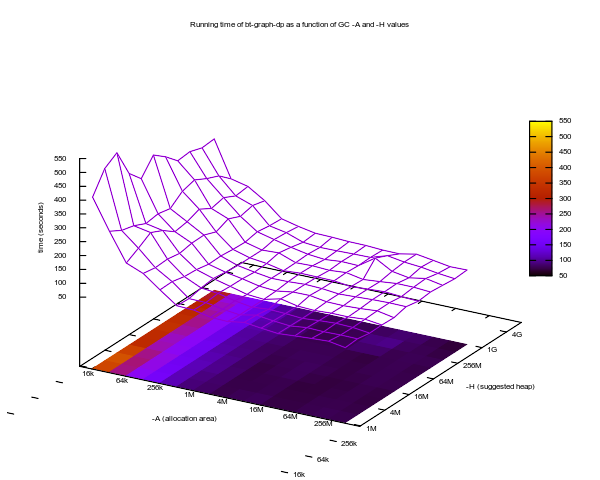
\includegraphics{bt-graph-dp-time-gc-space}
  }
\caption[{[EE] $\dpbt$ Finding Optimal Memory Setup}]{This figure shows the results obtained after running \acrshort{dpbt} with the \texttt{ghc-gc-tune} tool in order to find the suboptimal configuration for Memory allocation. $y$ axis shows the total execution time, $x$ axis is the \texttt{-A} configuration flag and $z$ axis is the \texttt{-H} configuration flag.}
\label{fig:exp:opt-mem}
\end{figure}

In \autoref{fig:exp:opt-mem} we can appreciate that the tool runs sereval times the same program with different configurations on flags \texttt{-A} and \texttt{-H} until if it finds a minimum. The dark blue shows the better performance where the curve find its minimum execution time. 
This indicates two possible suboptimal setup, either when \texttt{-A} is equal to \texttt{-H}, or either when \texttt{-A} is $\frac{1}{4}$ of the \texttt{-H}. For all our experiments we have selected the first option which \texttt{-A} is equal to \texttt{-H}, because choosing any of the two best combinations provides the same results as it can be seen in \autoref{fig:exp:opt-mem}.
It is important to remind the reader that \texttt{ghc-gc-tune} \cite{ghctune} uses an heuristic algorithm, providing suboptimal results.

\section{Experimental Results}\label{sec:exp:observed-results}
\subsection{E1: Continuous behavior Analysis}\label{sub:sec:exp-1} 
\paragraph{Goal} In this experiment, we assess the ability of \acrshort{dpbt} to generate results incrementally.
In order to do that, we use the \acrfull{dm} Tool \emph{diefpy}~\cite{diefpy} which implements \emph{Diefficiency Metric}~\cite{diefpaper} measurement analysis.
This experiment allows us to answer research questions [R1] and [R3] defined in \qref{res:bt:question}. 

\paragraph{Procedure} We execute this experiment for each of the networks described in \autoref{data:set} and for each scenario described in \autoref{sub:exp:exp-data-setup}.
This experiment has been executed five times on each case until we found the proper vertex or edges in the selection described in \autoref{sub:exp:sel-vals}. The criteria followed by the selection of the vertices or edges are detailed in \autoref{sub:exp:sel-vals}.
The metric  \acrfull{dt}-described in \autoref{sub:metric}- is used to measure the continuous behavior of the proposed approach in a given time frame.
\autoref{table:e1:def} depicts the different configurations evaluated in this experiment.

\begin{table}[H]
  \centering
  \resizebox{1\textwidth}{!}{%
  \begin{tabular}{|p{0.25\linewidth}|c|c|c|c|}
    \hline
   \textbf{Network} & \textbf{Scenario ID} & \textbf{Exec Flags} & \textbf{Query} & \textbf{Timeout}\\
   \hline
   \multirow{9}{*}{Dbpedia} & E-H & \texttt{+RTS -A5G -N8 -c -H5G -RTS} & \texttt{by-edge (921, 4)} & 48 hours\\
   & E-L & \texttt{+RTS -A5G -N8 -c -H5G -RTS} & \texttt{by-edge (383, 397)} & 48 hours\\
   & E-M & \texttt{+RTS -A5G -N8 -c -H5G -RTS} & \texttt{by-edge (540, 60)} & 48 hours\\
   & VL-H & \texttt{+RTS -A5G -N8 -c -H5G -RTS} & \texttt{by-vertex 9} & 48 hours\\
   & VL-L & \texttt{+RTS -A5G -N8 -c -H5G -RTS} & \texttt{by-vertex 809} & 48 hours\\
   & VL-M & \texttt{+RTS -A5G -N8 -c -H5G -RTS} & \texttt{by-vertex 511} & 48 hours\\
   & VU-H & \texttt{+RTS -A5G -N8 -c -H5G -RTS} & \texttt{by-vertex 921} & 48 hours\\
   & VU-L & \texttt{+RTS -A5G -N8 -c -H5G -RTS} & \texttt{by-vertex 93} & 48 hours\\
   & VU-M & \texttt{+RTS -A5G -N8 -c -H5G -RTS} & \texttt{by-vertex 540} & 48 hours\\
   \hline
   \multirow{9}{*}{Moreno Crime} & E-H & \texttt{+RTS -A5G -N6 -c -H5G -RTS} & \texttt{by-edge (413, 419)} & 48 hours\\
   & E-L & \texttt{+RTS -A5G -N6 -c -H5G -RTS} & \texttt{by-edge (361, 19)} & 48 hours\\
   & E-M & \texttt{+RTS -A5G -N6 -c -H5G -RTS} & \texttt{by-edge (531, 196)} & 48 hours\\
   & VL-H & \texttt{+RTS -A5G -N6 -c -H5G -RTS} & \texttt{by-vertex 95} & 48 hours\\
   & VL-L & \texttt{+RTS -A5G -N6 -c -H5G -RTS} & \texttt{by-vertex 187} & 48 hours\\
   & VL-M & \texttt{+RTS -A5G -N6 -c -H5G -RTS} & \texttt{by-vertex 97} & 48 hours\\
   & VU-H & \texttt{+RTS -A5G -N8 -c -H5G -RTS} & \texttt{by-vertex 2} & 48 hours\\
   & VU-L & \texttt{+RTS -A5G -N6 -c -H5G -RTS} & \texttt{by-vertex 793} & 48 hours\\
   & VU-M & \texttt{+RTS -A5G -N6 -c -H5G -RTS} & \texttt{by-vertex 533} & 48 hours\\
   \hline
   \multirow{9}{*}{Opsahl UC Forum} & E-H & \texttt{+RTS -A5G -N6 -c -H5G -RTS} & \texttt{by-edge (213, 33)} & 48 hours\\
   & E-L & \texttt{+RTS -A5G -N6 -c -H5G -RTS} & \texttt{by-edge (398, 10)} & 48 hours\\
   & E-M & \texttt{+RTS -A5G -N6 -c -H5G -RTS} & \texttt{by-edge (129, 171)} & 48 hours\\
   & VL-H & \texttt{+RTS -A5G -N6 -c -H5G -RTS} & \texttt{by-vertex 289} & 48 hours\\
   & VL-L & \texttt{+RTS -A5G -N6 -c -H5G -RTS} & \texttt{by-vertex 258} & 48 hours\\
   & VL-M & \texttt{+RTS -A5G -N6 -c -H5G -RTS} & \texttt{by-vertex 433} & 48 hours\\
   & VU-H & \texttt{+RTS -A5G -N8 -c -H5G -RTS} & \texttt{by-vertex 395} & 48 hours\\
   & VU-L & \texttt{+RTS -A5G -N6 -c -H5G -RTS} & \texttt{by-vertex 390} & 48 hours\\
   & VU-M & \texttt{+RTS -A5G -N6 -c -H5G -RTS} & \texttt{by-vertex 207} & 48 hours\\
   \hline
   \multirow{9}{*}{Wang Amazon} & E-H & \texttt{+RTS -A5G -N6 -c -H5G -RTS} & \texttt{by-edge (839, 9)} & 48 hours\\
   & E-L & \texttt{+RTS -A5G -N6 -c -H5G -RTS} & \texttt{by-edge (10987, 36)} & 48 hours\\
   & E-M & \texttt{+RTS -A5G -N6 -c -H5G -RTS} & \texttt{by-edge (19630, 84)} & 48 hours\\
   & VL-H & \texttt{+RTS -A5G -N6 -c -H5G -RTS} & \texttt{by-vertex 124} & 48 hours\\
   & VL-L & \texttt{+RTS -A5G -N6 -c -H5G -RTS} & \texttt{by-vertex 321} & 48 hours\\
   & VL-M & \texttt{+RTS -A5G -N6 -c -H5G -RTS} & \texttt{by-vertex 64} & 48 hours\\
   & VU-H & \texttt{+RTS -A5G -N8 -c -H5G -RTS} & \texttt{by-vertex 1727} & 48 hours\\
   & VU-L & \texttt{+RTS -A5G -N6 -c -H5G -RTS} & \texttt{by-vertex 9970} & 48 hours\\
   & VU-M & \texttt{+RTS -A5G -N6 -c -H5G -RTS} & \texttt{by-vertex 73} & 48 hours\\
   \hline
  \end{tabular}
  }
 \caption[{[EE] E1 Procedure}]{This table shows all the different experiments setups conducted for E1. Execution flags are the Runtime execution flags which needs to be set on the execution command as it is detailed in \autoref{apx:running:experiments}. On the last column we can see for each scenario, the query command executed for \acrshort{bt} enumeration (see \dref{def:query:match})}
 \label{table:e1:def}
 \end{table}

 \paragraph{Observed Results}\label{sub:sec:res:e1}
 As observed in the results above in \autoref{fig:dief:dbpedia}, \autoref{fig:dief:moreno}, \autoref{fig:dief:opsahl} and \autoref{fig:dief:wang} in all the networks and experiments setups, \acrshort{bt} are incrementally enumerated and delivered. 

 \begin{figure}[!htp]
  \centering
  \begin{subfigure}[t]{0.45\textwidth}
   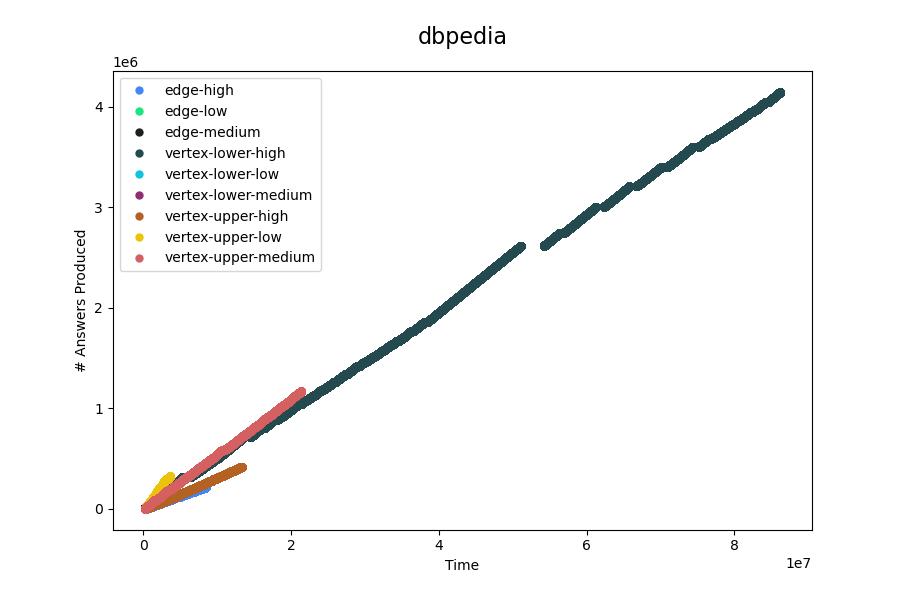
\includegraphics[width=1\linewidth, height=0.2\textheight]{experiments/diepfy/dbpedia.png}
    \caption[{[EE] \acrshort{dm} Results: \acrshort{dbpedia}}]{\acrshort{dm} metric results after running all experiment scenarios described in \autoref{table:e1:def} on the DBpedia network. Each color represents one scenario}
    \label{fig:dief:dbpedia}
  \end{subfigure}\hfill
  \begin{subfigure}[t]{0.45\textwidth}
   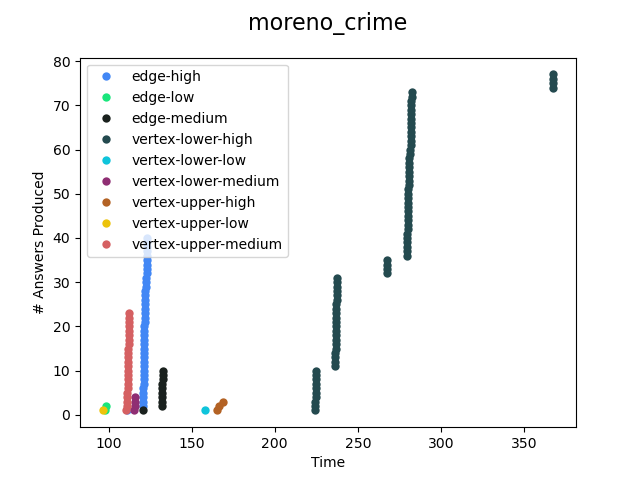
\includegraphics[width=1\linewidth, height=0.2\textheight]{experiments/diepfy/moreno_crime.png}
    \caption[{[EE] \acrshort{dm} Results: Moreno Crime}]{\acrshort{dm} metric results after running all experiment scenarios described in \autoref{table:e1:def} on Moreno Crime network. Each color represents one scenario}
    \label{fig:dief:moreno}
  \end{subfigure}
  \vspace{0.5cm}

  \begin{subfigure}[t]{0.45\textwidth}
   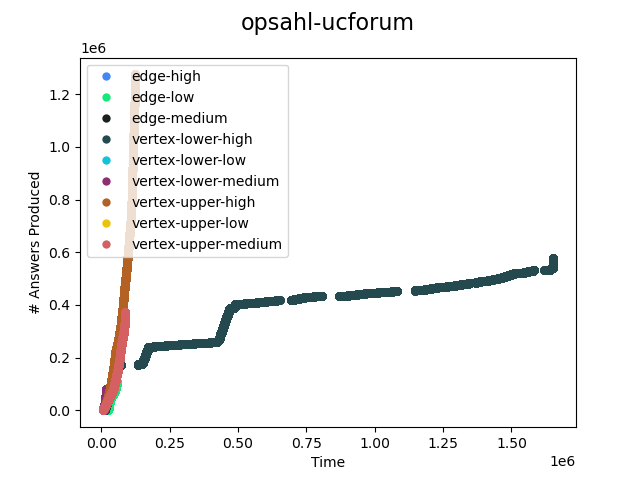
\includegraphics[width=1\linewidth, height=0.2\textheight]{experiments/diepfy/opsahl-ucforum.png}
    \caption[{[EE] \acrshort{dm} Results: Opsahl UC Forum}]{\acrshort{dm} metric results after running all experiment scenarios described in \autoref{table:e1:def} on Opsahl UC Forum network. Each color represents one scenario}
    \label{fig:dief:opsahl}
  \end{subfigure}\hfill
  \begin{subfigure}[t]{0.45\textwidth}
    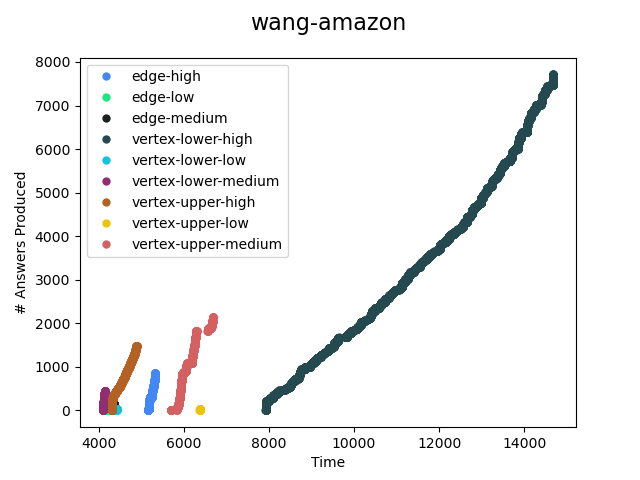
\includegraphics[width=1\linewidth, height=0.2\textheight]{experiments/diepfy/wang-amazon.png}
     \caption[{[EE] \acrshort{dm} Results: Wang Amazon}]{\acrshort{dm} metric results after running all experiment scenarios described in \autoref{table:e1:def} on Wang Amazon network. Each color represents one scenario}
     \label{fig:dief:wang}
   \end{subfigure}
   \caption[{[EE] \acrshort{dm} General Results}]{These figures show \acrshort{dm} observed results after running all the scenarios described in \autoref{table:e1:def} for each network. $y$ axis represents the number of Answers produced and $x$ axis is the $t$ time of the \acrshort{dm} metric describe in \autoref{sub:metric}. For example in \autoref{fig:dief:dbpedia} we can see that dark green color shows VL-H scenario on DBpedia network. The more data points distributed throughout the $x$ axis, the higher, the continuous behavior.}
   \label{fig:dief:all}
 \end{figure}

The continuous behavior can be appreciated in \autoref{fig:dief:all} having the fact that any of those points draw a straight vertical line. 
If that were the case, the plot would have indicated that all the $t$ times, in \acrshort{dm} metric, are being produced at the same $t$.
Moreover we can observed \acrshort{dm} values for dbpedia of $4, 1.22, 6, 9.8, 1.14, 6.32, 4.11, 8.15$ and $3.63$ for the nine scenarios indicating continuous behavior. 
In the case of Opsahl UC Forum \acrshort{dm} of $5, 1.51, 10, 7.68, 4.30, 3.23, 1.06, 8.48, 5.77$ indicating continuous behavior as well.
Having those values, we can ensure that all the results are continuously generated by \acrshort{dpbt}.
We can also observe how the results obtained in experiments VU-M for Opshal with $10$, e-L for Moreno with $28.42$, VL-M for dbpedia with $9.8$ and VL-M for Wang Amazon with $11766.99$ (see \autoref{table:exp:data-setup}), are more continuous compare to the rest of the experiments setups. 
The only experiment setup that cannot be appreciated with the same level of continuous results as the rest is \emph{Wang Amazon} which for the rest of the scenarios has value $0$ of \acrshort{dm} metric. 
Moreover, it is observed how Moreno Crime in \autoref{fig:dief:moreno} that between time $100$ and $150$, scenarios VL-H, VL-M, and VL-L are plotting in the same $t$ all the enumerated \acrshort{bt}, with a \acrshort{dm} value of $0$ indicating low continuous behavior. 
This network is the only one exhibiting that behavior in more than two scenarios.

\begin{figure}[!htp]
  \centering
  \begin{subfigure}[t]{0.45\textwidth}
  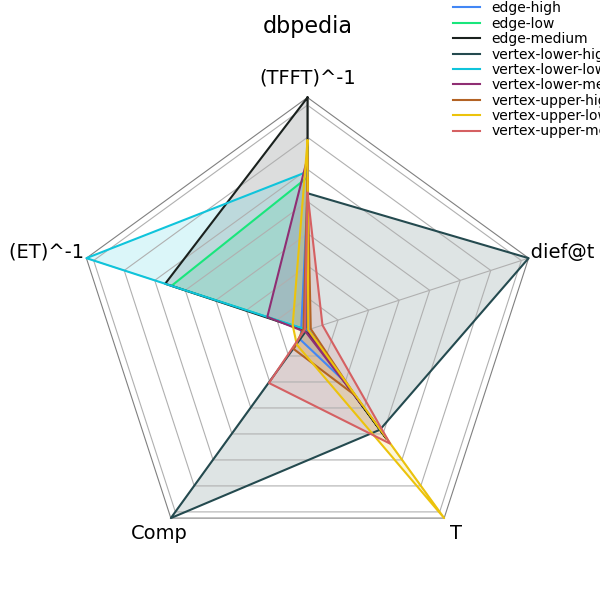
\includegraphics[width=1\linewidth, height=0.25\textheight]{experiments/diepfy/dbpedia_radial.png}
    \caption[{[EE] \acrshort{dm} Results (Radial): \acrshort{dbpedia}}]{\acrshort{dm} metric results in radial plot after running all experiment scenarios described in \autoref{table:e1:def} on DBpedia network. Each color represents one scenario. Each dimension of the radial represents an observed result for that scenario on that dimension}
    \label{fig:dief:dbpedia-radial}
  \end{subfigure}\hfill
  \begin{subfigure}[t]{0.45\textwidth}
  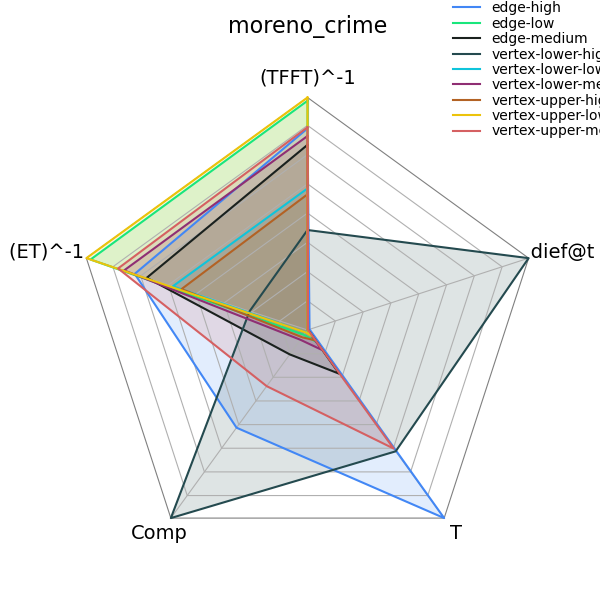
\includegraphics[width=1\linewidth, height=0.25\textheight]{experiments/diepfy/moreno_crime_radial.png}
    \caption[{[EE] \acrshort{dm} Results (Radial): Moreno Crime}]{\acrshort{dm} metric results in radial plot after running all experiment scenarios described in \autoref{table:e1:def} on Moreno Crime network. Each color represents one scenario. Each dimension of the radial represents an observed result for that scenario on that dimension}
    \label{fig:dief:moreno-radial}
  \end{subfigure}
  \vspace{0.5cm}
  %
  \begin{subfigure}[t]{0.45\textwidth}
  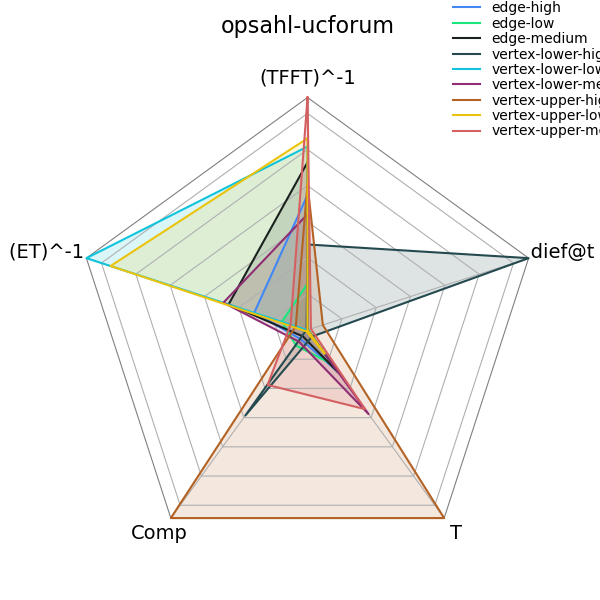
\includegraphics[width=1\linewidth, height=0.25\textheight]{experiments/diepfy/opsahl-ucforum_radial.png}
    \caption[{[EE] \acrshort{dm} Results (Radial): Opsahl UC Forum}]{\acrshort{dm} metric results in radial plot after running all experiment scenarios described in \autoref{table:e1:def} on Opsahl UC Forum network. Each color represents one scenario. Each dimension of the radial represents an observed result for that scenario on that dimension}
    \label{fig:dief:opsahl-radial}
  \end{subfigure}\hfill
  \begin{subfigure}[t]{0.45\textwidth}
    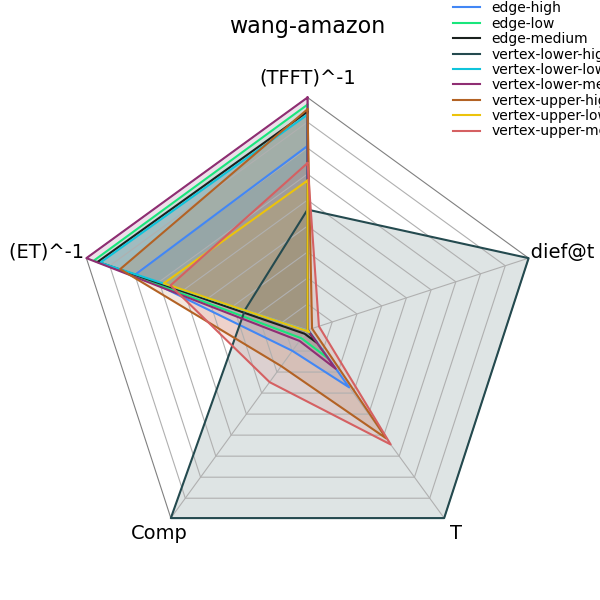
\includegraphics[width=1\linewidth, height=0.25\textheight]{experiments/diepfy/wang-amazon_radial.png}
    \caption[{[EE] \acrshort{dm} Results (Radial): Wang Amazon}]{\acrshort{dm} metric results in radial plot after running all experiment scenarios described in \autoref{table:e1:def} on Wang Amazon network. Each color represents one scenario. Each dimension of the radial represents an observed result for that scenario on that dimension}
    \label{fig:dief:wang-radial}
  \end{subfigure}
  \caption[{[EE] \acrshort{dm} General Results (Radial)}]{Radial plots show how the different dimensions values provided by \acrshort{dm} tool such as \acrfull{tt}, \acrfull{tfft}, \acrfull{dt}, \acrfull{et} and \acrfull{comp} are related each other for each experimental case. These figures show radial plot observed results after running all the scenarios described in \autoref{table:e1:def} for each network. \acrshort{dm} is described in \\ \autoref{sub:metric}.}
\end{figure}

Another plots that \acrshort{dm} tool provides are shown in \autoref{fig:dief:dbpedia-radial}, \autoref{fig:dief:moreno-radial}, \autoref{fig:dief:opsahl-radial} and \autoref{fig:dief:wang-radial}.
Here we can observe how all the networks under the VL-H scenario cover \acrshort{dt} metrics with the dark green area, which indicates that it is continuously delivering results for each network. 
The rest of the data setup experiments indicates that the level of throughput, completeness, and execution time is less than \acrfull{dt}, and the results can be delivered faster without appreciating continuous behavior properly in the plot. 
These radial plots obtained from \acrshort{dm} shows how \acrfull{et}, \acrfull{tfft}, \acrfull{comp}, \acrfull{tt} and \acrshort{dm} measured by tool, relate each other in the same setup. 
For our case analysis, the higher the area that is cover in \acrfull{dt} the better, indicating a high level of continuous behavior.

\subsection{E2: Benchmark Analysis}\label{sub:sec:exp-2} 
\paragraph{Goal} Regarding benchmarking, we aim at answering research question [R2] and assess  the impact of the type of command query $Q$ on the  \acrshort{bt} enumeration.
The results of this evaluation will also provide evidence to answer [R3] since we have provided evidence with the benchmarking that the execution time varies depending on the command query $q$ proving that we are effectively implemented a \emph{pay-as-you-go} model. 

\paragraph{Procedure} This experiment measures \emph{Average Running Time} and \emph{Total Running Time} as  described in \autoref{sub:metric}. 
For gathering \emph{Average Running Time}, the experiment scenarios described in \autoref{table:e2:def} were conducted; the \emph{\acrshort{dbpedia}} network was not considered, but the \mintinline{shell}{criterion} \cite{criterion} benchmark tool were followed.
The command run for \texttt{criterion} benchmark analysis is \mintinline[fontsize=\small, breaklines]{bash}{stack exec benchmark}. 

\begin{table}[H]
\centering
\begin{tabular}{|c|c|c|c|}
  \hline
  \textbf{Network} & \textbf{Scenario ID} & \textbf{Query} & \textbf{Timeout}\\
  \hline
  \multirow{9}{*}{Moreno Crime} & E-H & \texttt{by-edge (413, 419)} & 48 hours \\
  & E-L & \texttt{by-edge (361, 19)} & 48 hours \\
  & E-M & \texttt{by-edge (531, 196)} & 48 hours \\
  & VL-H & \texttt{by-vertex 95} & 48 hours \\
  & VL-L & \texttt{by-vertex 187} & 48 hours \\
  & VL-M & \texttt{by-vertex 97} & 48 hours \\
  & VU-H & \texttt{by-vertex 2} & 48 hours \\
  & VU-L & \texttt{by-vertex 793} & 48 hours \\
  & VU-M & \texttt{by-vertex 533} & 48 hours \\
  \hline
  \multirow{9}{*}{Opsahl UC Forum} & E-H & \texttt{by-edge (213, 33)} & 48 hours \\
  & E-L & \texttt{by-edge (398, 10)} & 48 hours \\
  & E-M & \texttt{by-edge (129, 171)} & 48 hours \\
  & VL-H & \texttt{by-vertex 289} & 48 hours \\
  & VL-L & \texttt{by-vertex 258} & 48 hours \\
  & VL-M & \texttt{by-vertex 433} & 48 hours \\
  & VU-H & \texttt{by-vertex 395} & 48 hours \\
  & VU-L & \texttt{by-vertex 390} & 48 hours \\
  & VU-M & \texttt{by-vertex 207} & 48 hours \\
  \hline
  \multirow{9}{*}{Wang Amazon} & E-H & \texttt{by-edge (839, 9)} & 48 hours \\
  & E-L & \texttt{by-edge (10987, 36)} & 48 hours \\
  & E-M & \texttt{by-edge (19630, 84)} & 48 hours \\
  & VL-H & \texttt{by-vertex 124} & 48 hours \\
  & VL-L & \texttt{by-vertex 321} & 48 hours \\
  & VL-M & \texttt{by-vertex 64} & 48 hours \\
  & VU-H & \texttt{by-vertex 1727} & 48 hours \\
  & VU-L & \texttt{by-vertex 9970} & 48 hours \\
  & VU-M & \texttt{by-vertex 73} & 48 hours \\
  \hline
\end{tabular}
\caption[{[EE] E2 Procedure}]{This table shows all the different experiments setups that we have conducted for E2. Execution command is the same for each experiment because it is handled by \texttt{criterion} tool. On the last column we can see for each scenario the query command executed for \acrshort{bt} enumeration (see \dref{def:query:match}), although the output is not used in this case, because we focus on average running time}
\label{table:e2:def}
\end{table}

Furthermore, \emph{Total Running Time} is gathered with the time measured after running all the scenarios described in \autoref{table:e1:def}.


\paragraph{Observed Results}\label{sub:sec:res:e2} As it can be seen in \autoref{fig:exp:bench}, yellow bars are all the experiments related to Lower Layer vertices, blue bars are related to Upper Layer, and red bars are the experiments related to edge search. 
The longest bars are from network opsahl-ucforum, which we already know by \autoref{table:exp:data-set} it is the biggest of the four networks in terms of the number of \acrshort{bt} and wedges. So, it needs to enumerate more \acrshort{bt}. 
Further, almost all the high incidence vertices and edges queries are taken longer as well. 
There is only one scenario that behaves differently, which is edges (see \autoref{table:exp:data-setup}) for opsahl-ucforum, where execution time is not proportional to incidence level.

\begin{figure}[!htb]
 \begin{center}
    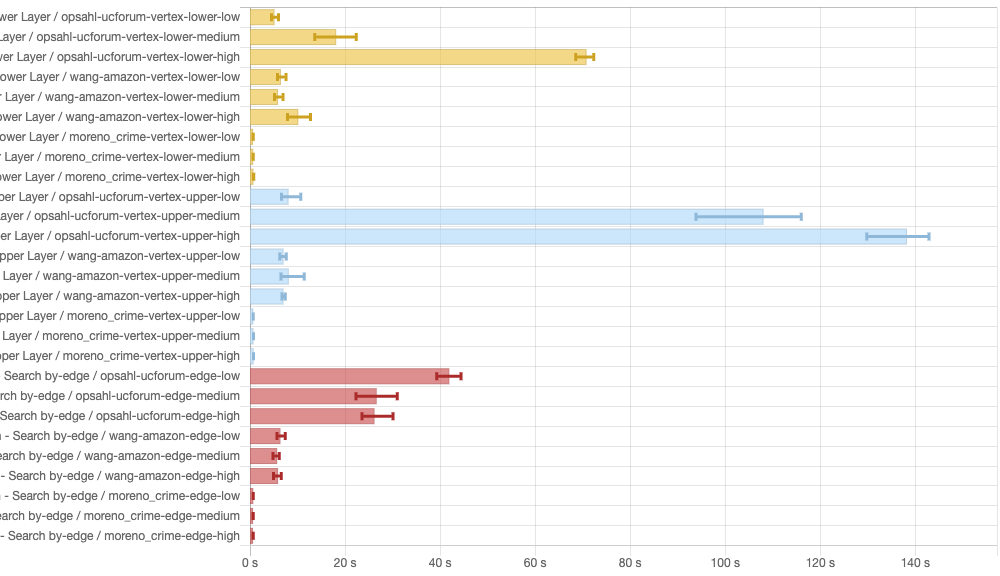
\includegraphics[width=1\textwidth] {experiments/bench_1}
      \end{center}
    \caption[{[EE] Benchmark Results: Criterion Plot}]{This plot depicts the results after running \texttt{criterion} the tool over the experimental setup described in \autoref{table:e2:def}. Yellow bars are the experiments over Opsahl UC Forum network. Blue light bars represents the experiments on Moreno Crime network, and red bars on Wang Amazon}
    \label{fig:exp:bench}
\end{figure}

 The \emph{Total Running Time}, which can be seen in \autoref{fig:exp:bench:2}, is also reported.

\begin{figure}[!htb]
  \begin{center}
     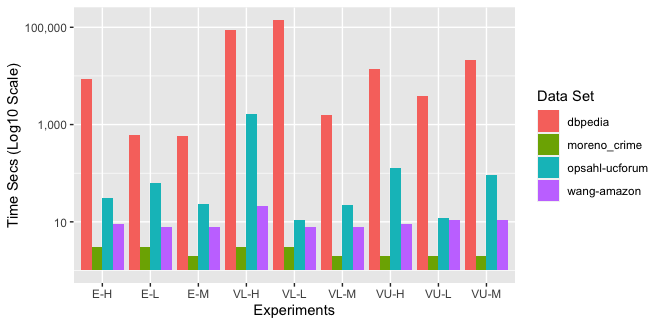
\includegraphics[width=1\textwidth] {experiments/execution_time_by_experiments}
       \end{center}
     \caption[{[EE] Total Execution Time: Comparison between all setups}]{This plot shows all the experiment scenarios run in \autoref{table:e1:def} and the comparison of the Total running execution time for each case. $y$ axis shows the total time in $\ln$ scale and $x$ axis is each Scenario ID describe in \autoref{table:exp:data-setup}}
     \label{fig:exp:bench:2}
 \end{figure}

Regarding \autoref{fig:exp:bench:2}, it is observed with the red bars that \acrshort{dbpedia} was the one which took more time in all scenarios.
We can also see in \autoref{fig:exp:bench:2} that scenario E-H took $8756$ seconds in \acrshort{dbpedia} network compare with the E-L and E-M, which took $596$ seconds and $577$ seconds, respectively. 
Also, in \autoref{fig:exp:bench:2}, we can see that Opsahl UC Forum took $1660$ seconds for VL-H scenario, $11$ seconds for VL-L, and $22$ seconds for VL-M, also showing the same behavior as \acrshort{dbpedia}.
Moreover, in \autoref{fig:exp:bench:2} it can also be appreciated how Wang Amazon network and Moreno Crime are showing the same behavior for VL-H, VL-L, and VL-M scenarios, where Wang Amazon networks report $21, 8$ and $8$ seconds, respectively and Moreno Crime $3, 3$ and $2$ seconds.
The same behavior repeats for all networks and all scenarios, indicating that the experiments with higher incidence take more time to finalize the execution compared to the experiments with lower incidence. This means that the type of query command $Q$ impacts on the execution of the program; the higher the incidence, the more bi-triangles to be enumerated and the longest the program will take to finish.

\subsection{E3: Performance Analysis}\label{sub:sec:exp-3} 
\paragraph{Goal} In this experiment, we take measurements on one network, to gather data about the use of memory allocation and threads on \acrshort{ghc} during the execution of \acrshort{dpbt}.

\paragraph{Procedure} This experiment gathers three metrics describe in \autoref{sub:metric}: \emph{GHC Productivity}, \emph{Distribution of Threads per Core} and \emph{Distribution of Allocated Memory per Data Type}.
Using \mintinline{shell}{ThreadScope} \cite{threadscope} tool we measure \emph{GHC Productivity}, \emph{Distribution of Threads per Core}, and using \mintinline{shell}{eventlog2html} \cite{eventlog2html} tool, we measure \emph{Distribution of Allocated Memory per Data Type}.
For both cases, we have run these tools using one network only and one scenario. This is because both tools enable profiling flags at compilation level on \acrshort{ghc}, penalizing performance.

\begin{table}[H]
\centering
\resizebox{1\textwidth}{!}{%
\begin{tabular}{|c|c|c|c|c|c|}
  \hline
  \textbf{Tool} & \textbf{Network} & \textbf{Scenario ID} & \textbf{Exec Flags} & \textbf{Query} & \textbf{Timeout}\\
  \hline
  \texttt{ThreadScope} & Dbpedia & VU-L & \texttt{+RTS -A10G -H10G -c -N8 -l -s -RTS} & \texttt{by-vertex 93} & 24 hours\\
  \hline
  \texttt{eventlog2html} & Dbpedia & VU-L & \texttt{+RTS -A10G -H10G -c -N8 -l -s -RTS} & \texttt{by-vertex 93} & 24 hours\\
  \hline
\end{tabular}
}
\caption[{[EE] E3 Procedure}]{This table shows the experiments scenario run for each of the tools. Notice the increase of \texttt{-A} and \texttt{-H} to support more memory allocation due to the profiling analysis}
\label{table:e3:def}
\end{table}

As observed in \autoref{table:e3:def}, although we have selected the biggest network, we are only running the tools to gather data using VU-L, which enumerate less \acrshort{bt}. Therefore, this allows for the retrieval of profiling information, such as multithreading details and memory allocation.

\paragraph{Observed Results}\label{sub:sec:res:e3}
We can divide the analysis of this section into two: memory consumption and multithreading.

\paragraph{Multithreading} Regarding multithreading, we have gathered multithreading metrics of different time slots of the total execution time of Moreno Crime network run.
We could not analyze bigger networks due to the huge amount of data gathered that make the program timeout for this experiment. The timeout on this case was set on $24$ hours and the program timed out running out of memory.
As we can see in the overview, execution in \autoref{fig:exp:perf:1} all the cores (8) are running \acrfull{mut} time in threads almost during the whole execution of the program.
Running \acrfull{mut} most of the execution of the program, also indicates that there are few GC pauses, and running time is overtaken by \acrshort{mut} time and not GC. In fact, \acrshort{ghc} productivity on this run indicated $99.8\%$.
\begin{figure}[!htb]
  \centering
  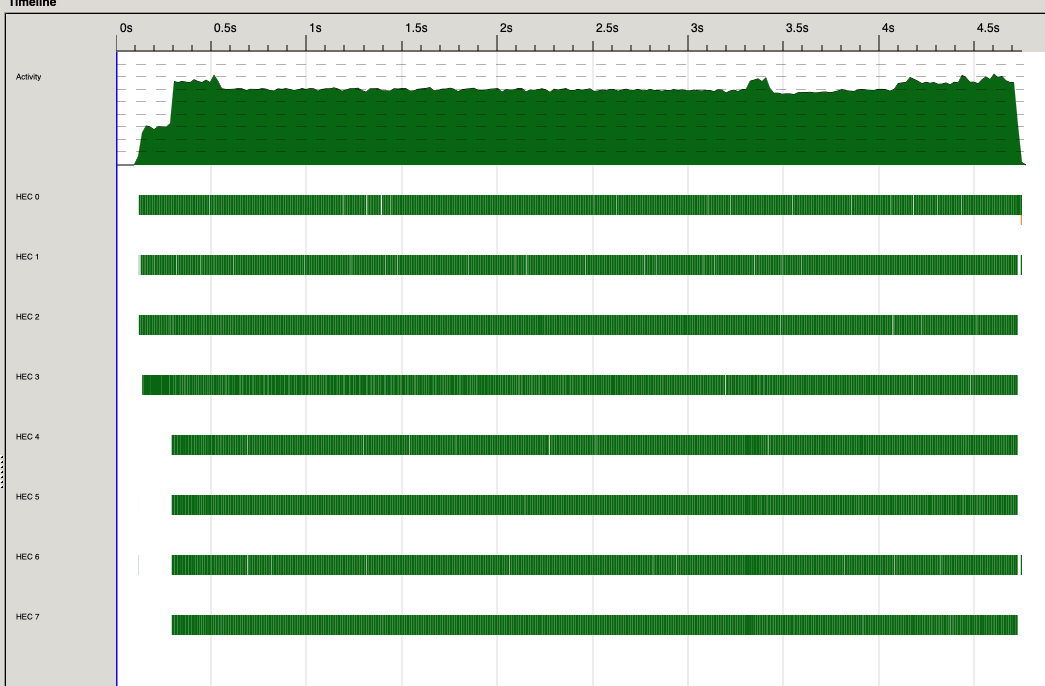
\includegraphics[width=1\textwidth]{experiments/thread/general_overview}
  \caption[{[EE] Thread Metrics: General overview}]{This is a general overview of ThreadScope results over the experiments running. Green bar indicates \acrshort{mut} time. The distribution between different 8 green bars means that it is executing on the 8 assigned cores.}
  \label{fig:exp:perf:1}
 \end{figure}

ThreadScope~\cite{threadscope} output allows us to zoom in different portions of the execution time to analyze the results better. 
If we zoom in on the execution threads at the beginning and at the end, we are going to see that there is a moment when only one core is executing. 
At the middle of the execution, we are seeing more processing distributing evenly among cores with less use GC and higher \acrshort{mut} time.

\begin{figure}[!htb]
  \centering
  \begin{subfigure}[t]{0.3\textwidth}
   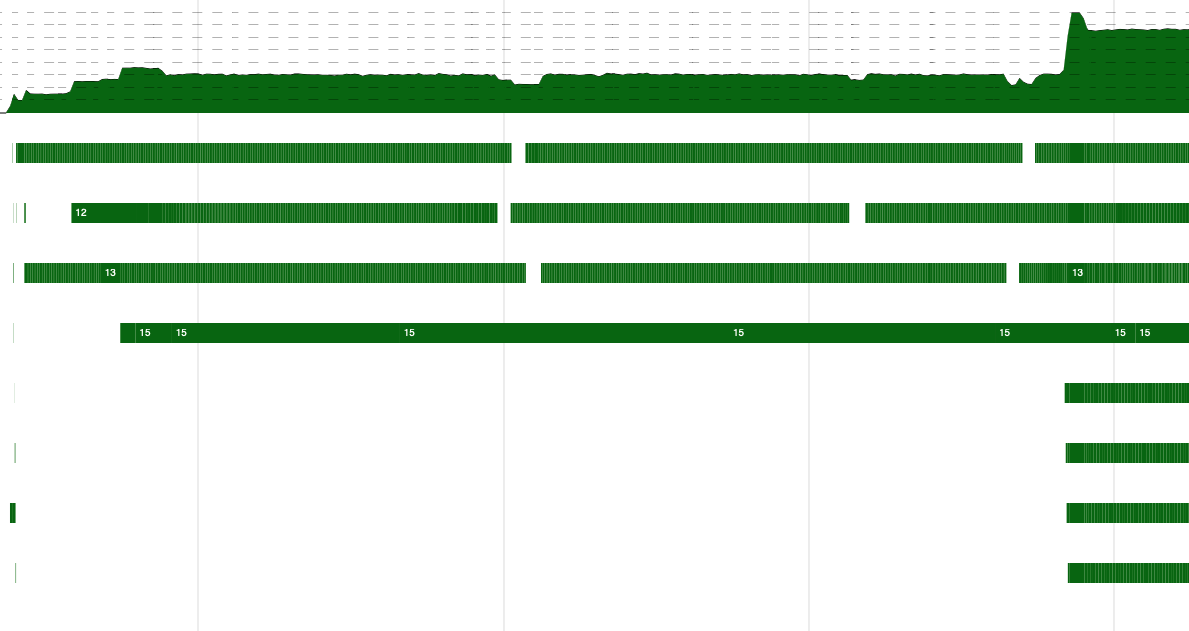
\includegraphics[width=1\linewidth, height=0.2\textheight]{experiments/thread/init}
   \caption{{[EE] Thread Metrics: Initial execution}}
   \label{fig:exp:perf:2}
  \end{subfigure}%
  \hspace{.3cm}%
  \begin{subfigure}[t]{0.3\textwidth}
    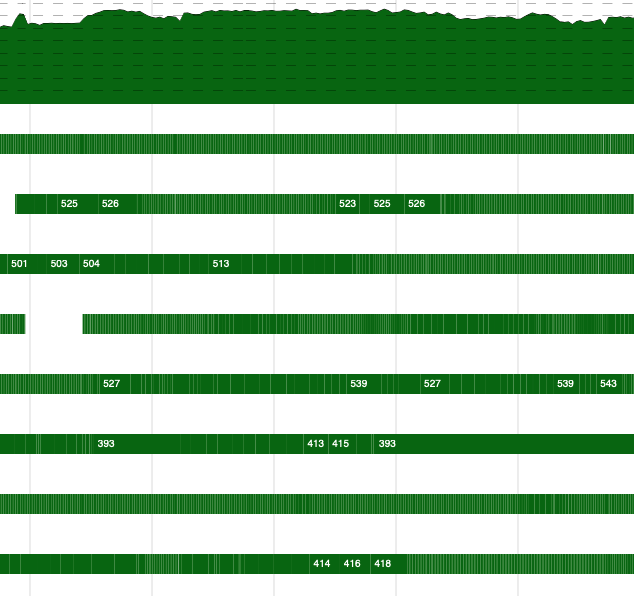
\includegraphics[width=1\linewidth, height=0.2\textheight]{experiments/thread/middle}
    \caption{{[EE] Thread Metrics: Middle of execution}}
    \label{fig:exp:perf:4}
   \end{subfigure}% 
   \hspace{.3cm}%
   \begin{subfigure}[t]{0.3\textwidth}
   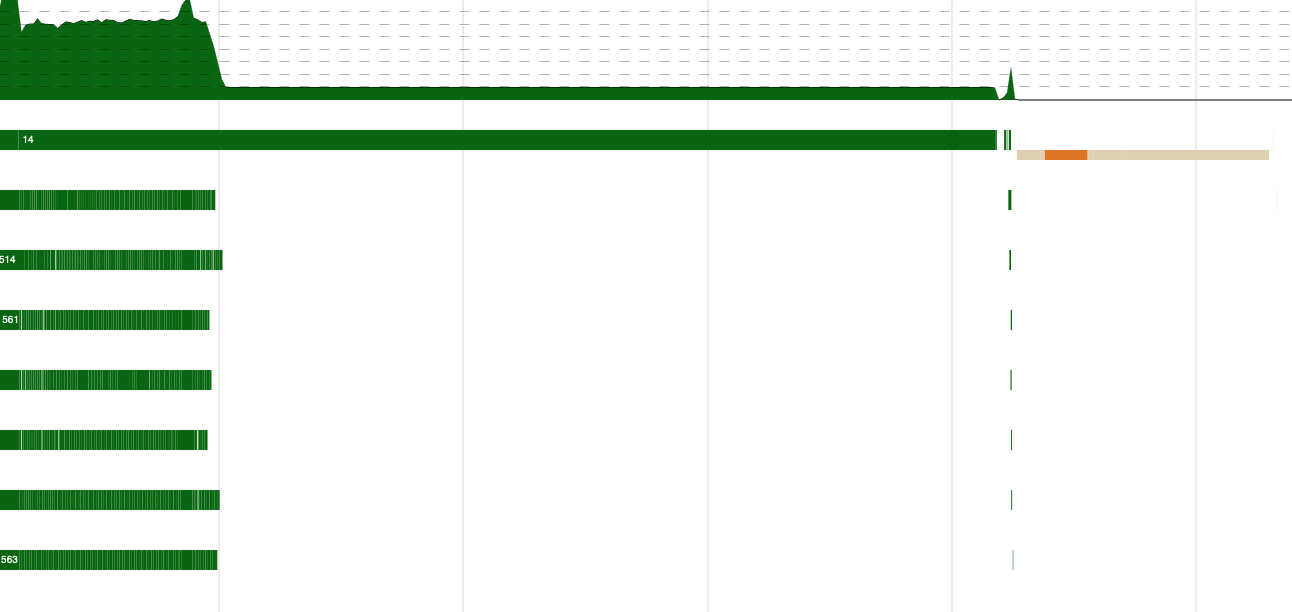
\includegraphics[width=1\linewidth, height=0.2\textheight]{experiments/thread/end}
   \caption{{[EE] Thread Metrics: End of execution}}
   \label{fig:exp:perf:3}
  \end{subfigure}%
  \caption[{[EE] Thread Metrics: Partitioned}]{These plots depict different moments of the execution of the program after doing a zoom of the images allowing to scale down execution time view. The left image indicates the beginning of the execution. Middle image is the middle of the execution and right image is the end of the execution.}
\end{figure}

\paragraph{Memory Consumption} In the case of memory consumption, we have been able to measure the memory consumption for the biggest graph, \acrshort{dbpedia}. 
As it is known, enabling profiling downgrades the performance of execution time. Because of that, the program runs out of memory after $24$ hs., as we are going to see in the image. Although this, we have still been able to gather memory allocation data to conduct the analysis.

\begin{figure}[!htb]
  \begin{center}
     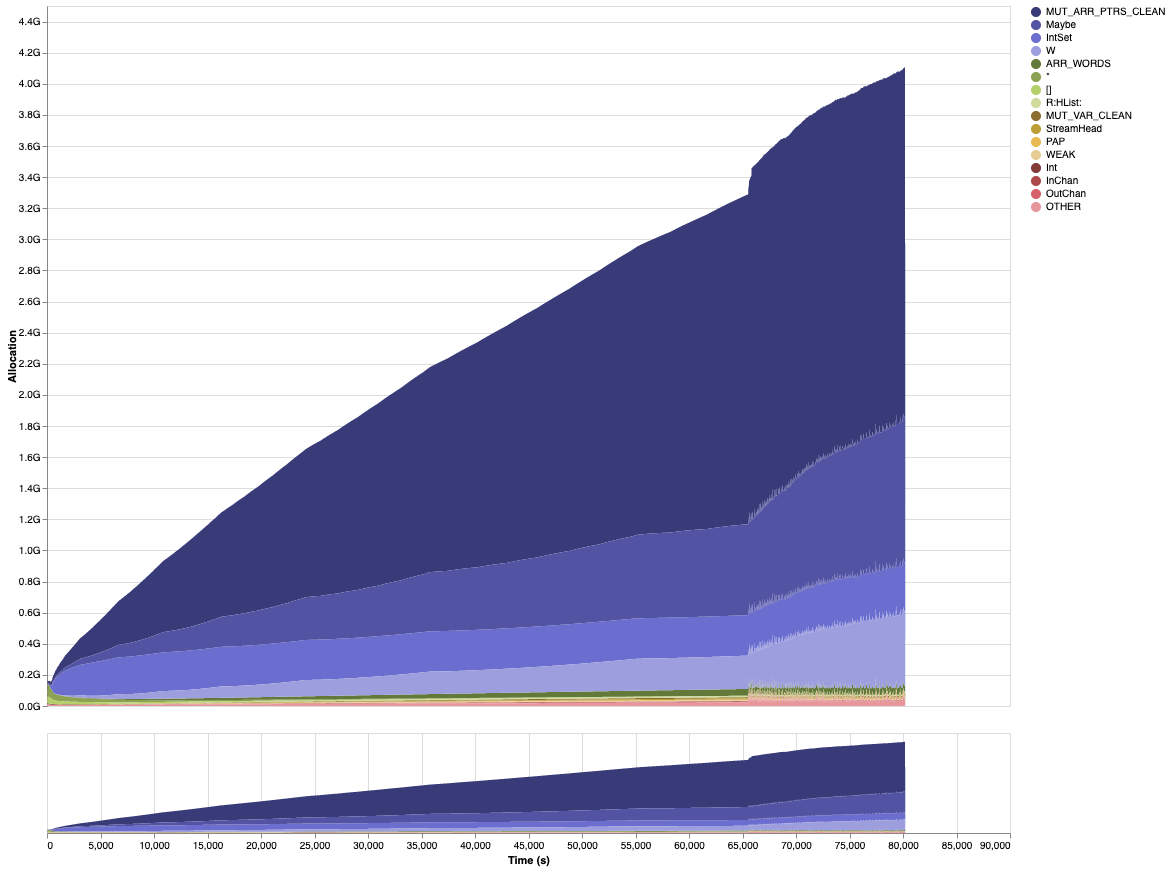
\includegraphics[width=1\textwidth] {experiments/mem/overview}
       \end{center}
     \caption[{[EE] Memory Metrics: Allocation by Data Type}]{This plot is showing the accumulated memory allocation size of each \acrshort{hs} Data Type throughout the execution of the program.}
     \label{fig:exp:mem:1}
 \end{figure}

As we can appreciate in \autoref{fig:exp:mem:1} the darkest blue area belongs to \texttt{MUT\_ARR\_PTRS\_CLEAN}. These types of objects are pointers to function.
It is clear that \texttt{MUT\_ARR\_PTRS\_CLEAN} is allocating $2G$ at most, and it is more than the rest of the objects. This also represents more than $50\%$ of the accumulated memory allocation during the whole execution time.
Below dark blue \texttt{MUT\_ARR\_PTRS\_CLEAN}, there is a lighter blue area, which represents the allocation of \texttt{Maybe} type. \texttt{Maybe} is the type that transfers data between stages through channels. It also represents the $25\%$ of the total allocated memory with less than $1G$ in total.
Continue below \texttt{Maybe} type, it is \texttt{IntSet} data type memory allocation, which is the type for storing the \acrshort{adwg} and \acrshort{abt} as we have described on \autoref{sec:prem:def}. This is even lower than the previous one, allocating up to $0.3G$ of memory that does not represent more than $7\%$ of the total memory. 
Alongside this, it is the \texttt{W} type which is storing \acrshort{awg}; it represents $0.5G$ which is a $10\%$ of the total allocation.
The rest $10\%$ of the total memory is evenly distributed among other data types that are not part of the specific \acrshort{dpfh} implementation, but from \acrshort{hs} in general.
 
\section{Discussion}\label{sec:exp:discussion}
\paragraph{E1: Continuous behavior} \autoref{sub:sec:res:e1} reports show that continuous behavior can be appreciated better in some scenarios and networks than others. For example, the scenarios containing queries with lower and medium incident vertices. 
The behavior on these cases can be explained because bi-triangles are aggregated based on triple $\ell = (l_l,l_m,l_u)$ (see \dref{def:abt}). Then, if the requested $l \in L$ matches with some of these vertices in $\ell$, all the $\hat{U}_l$ cartesian product need to be enumerated in a 6-cycle path \acrshort{bt} (see \dref{def:bt}). 
Therefore, if there are few \acrshort{bt} because the incidence level is lower, this is going to be delivered faster and continuously.
Moreover, the cases that exhibit less continuous behavior are Wang Amazon and Moreno Crime networks in the majority of their scenarios. In the case of Wang Amazon $8$ out of $9$ scenarios shows a \acrshort{dm} value of $0$. In the case of Moreno crime networks, it is reported a \acrshort{dm} value of $0$ in $5$ out of $9$ scenarios. 
We provide two arguments that support the explanation of this low continuous level in Wang Amazon and Moreno Crime. 
Firstly, the selection of the command $Q$ value (vertex or edge) for the different experimental scenario is \emph{pseudo-random}-- as it is commented in \autoref{sub:exp:sel-vals}. 
We have detected that for this particular experiment setup, even when the \emph{pseudo-randomly} chosen vertex belongs to the Lower Layer $L$, it is not a vertex with a high incidence as it should be.
Secondly, it could be explained by the fact of the topology of both graphs. Wang Amazon and Moreno Crime networks are the smallest of all the graphs used, in terms of the number of \acrshort{bt} as we can see in \autoref{table:exp:data-set}.
Therefore, results are delivered extremely fast and incremental results only can be appreciated in the vertices with high incidence.
In conclusion, we are able to answer [R1] and asses that we have built an incremental algorithm for enumerating \acrlong{bt}. 
The same conclusion can be obtained regarding question [R3]. We verify that, depending on the incidence of the vertex or edge, \acrshort{dpbt} is enumerating \acrshort{bt} in a continuous manner. This shows us \acrshort{dpbt} effectively implements a \emph{pay-as-you-go} model.

\paragraph{E2: Benchmark} Regarding \autoref{sub:sec:res:e2} we have noticed that for the case of edges scenarios in Opshal UC Forum network, the execution time is not consistent with what we expected regarding the incidence level. This could be explained by the \emph{pseudo-randomly} selection detailed in \autoref{sub:exp:sel-vals}.
In what relates to \emph{Total Execution time}, we have pointed out that DBpedia network is the one taking longer. This is perfectly explained by the characteristics and topology of the graph, since it is both the biggest graph in terms of edges and vertex, and it is the graph which proportionally has more \acrshort{bt}. 
We can answer the question [R2] because it can clearly be seen in the benchmark analysis and in \autoref{fig:exp:bench:2} that as long as the user request for command queries $Q$ that have more incidence in the graph and participates in more \acrshort{bt},
the execution time increases.


\paragraph{E3: Performance} In \autoref{sub:sec:res:e3} we have noticed the suitable distribution of threads among cores during the execution time. 
That exhibits a perfect fit with the \acrshort{dp} model since at the beginning, it considers all the filters and starts reading the input file, where there is less distribution of threads among the core. 
After that, we can see an even distribution and all cores busy when \acrshort{dp} executes the filters. Remember that each stage runs on its own thread. At the end, we observe a reduction in the distribution of the cores, because  the last part of the execution is done by $\obt$.
Regarding memory allocation, we have seen that most of the allocation is done by \texttt{MUT\_ARR\_PTRS\_CLEANER} data type.
In \acrlong{hs} \acrshort{mut} is the acronym of a thread evaluating an \acrshort{hs} expression.
Therefore, having $2G$ of allocated memory for \texttt{MUT\_ARR\_PTRS\_CLEANER} type means that there are many pointers allocated waiting for evaluating expressions. \acrshort{dpbt} implementation explains this behavior because it is spawning one
thread per stage, and in particular, that means one thread per filter instance as well. In the case of \acrshort{dbpedia} which contains $168.338$ vertices in 
$L$ according to \autoref{table:exp:data-set}, in the worst case \acrshort{dpbt} is spawning the same amount of threads for every run of this network. Since the execution of all these stages will not be released until it finishes the last $\ad$ (processing queries), all of them are waiting for the queries to be processed and executed.
Another important part of the allocated memory as we have seen in \autoref{sub:sec:exp-3} is distributed between \texttt{Maybe}, \texttt{IntSet} and \texttt{W} data types. This behavior is expected because \texttt{Maybe} carries data between stages which cannot be avoided due to the \acrshort{dp} model. Additionally,  both \texttt{IntSet} and \texttt{W} are the 
compressed form \acrshort{dpbt} uses for storing intermediate structures to build \acrshort{bt}, as we have described in \autoref{sec:prem:def}.
One of the proposed solutions for future work is to reduce the number of $\fbt$ for bigger graphs in order to reduce the number of allocated pointers waiting for commands.
Although memory allocation shows a linear growth in \autoref{fig:exp:mem:1} for the \texttt{MUT\_ARR\_PTRS\_CLEANER} type in this experiment, the rest of the memory allocation is not growing linearly, as we can see also in \autoref{fig:exp:mem:1}. This is a key factor on memory analysis since it is showing how \acrshort{dpfh} is compressing intermediate objects like \acrshort{awg}, \acrshort{adwg}, and \acrshort{abt} without penalizing the rest. 
In conclusion, we can answer the question [R4] as we have shown that threads are efficiently handled by \acrshort{hs} \acrshort{ghc} scheduler supporting the parallelization level that \acrshort{dp} requires. 
We can also state that memory management is efficiently handled as well by the analysis exposed before.
Additionally, memory allocation can be also improved by implementing a better matching algorithm for searching and deliver \acrshort{bt} like for example the ones describe by Lai et al.~\cite{Lai}. 
It was out of the scope of this work to solve the efficiency of the queries, as well as the underlying data structures improvements. 


\section{Chapter Summary}
In this chapter, we have explained the experiments conducted in order to answer our research question.
We first started presenting a summary of the research questions. After that, we have described the experimental configuration.
Then, the experimental procedure and results are reported. Finally, we have discussed the observed outcomes in terms of the main properties of our proposed approach.
To summarize, the main points observed during the experimentation are:
\begin{itemize}
  \item High values of the metric dief\@t that is indicating the continuous behavior of \acrshort{dpbt} exhibiting its capability of incrementally enumerates \acrshort{bt}.
  \item High values of the metrics \emph{Average Running Time} and \emph{Total Running Time} for scenarios which enumerates more bi-triangles, are suggesting an effective implementation of a \emph{pay-as-you-go} model of \acrshort{dpbt}.
  \item Results captured by the \texttt{ThreadScope} tool indicating an even distribution of the threads among processors, showing efficient use of the parallel model.
  \item Results gathered by the \texttt{eventlog2html} tool suggesting that memory consumption is efficiently handled in the intermediate objects that \acrshort{dpfh} collects on each filter and transfers between them. A proposal on how also improve this part was exposed in \autoref{sec:exp:discussion}.
\end{itemize} 
